\documentclass[conference]{IEEEtran}
\IEEEoverridecommandlockouts
% The preceding line is only needed to identify funding in the first footnote. If that is unneeded, please comment it out.
\usepackage{cite}
\usepackage{amsmath,amssymb,amsfonts}
\usepackage{algorithmic}
\usepackage{graphicx}
\usepackage{textcomp}
\usepackage{xcolor}
\usepackage[utf8]{inputenc}
\def\BibTeX{{\rm B\kern-.05em{\sc i\kern-.025em b}\kern-.08em
    T\kern-.1667em\lower.7ex\hbox{E}\kern-.125emX}}
\begin{document}

\title{Towards community and expert detection on open source global development}

\author{\IEEEauthorblockN{Vinicius Schettino}
\IEEEauthorblockA{\textit{Computer Science Postgraduate Program}\\
\textit{Federal University of Juiz de Fora}\\
Juiz de Fora, Brazil \\
vinicius.schettino@ice.ufjf.br}
\and
\IEEEauthorblockN{Vitor Horta}
\IEEEauthorblockA{\textit{Computer Science Postgraduate Program}\\
\textit{Federal University of Juiz de Fora}\\
Juiz de Fora, Brazil \\
vitor.horta@ice.ufjf.br}
\and
\IEEEauthorblockN{Marco Antônio P. Araújo}
\IEEEauthorblockA{\textit{Computer Science Postgraduate Program}\\
\textit{Federal University of Juiz de Fora}\\
Juiz de Fora, Brazil \\
marco.araujo@ufjf.edu.br}
\and
\IEEEauthorblockN{Victor Ströele}
\IEEEauthorblockA{\textit{Computer Science Postgraduate Program}\\
\textit{Federal University of Juiz de Fora}\\
Juiz de Fora, Brazil \\
victor.stroele@ufjf.edu.br}
}

\maketitle

\begin{abstract}
This document is a model and instructions for \LaTeX.
This and the IEEEtran.cls file define the components of your paper [title, text, heads, etc.]. *CRITICAL: Do Not Use Symbols, Special Characters, Footnotes,
or Math in Paper Title or Abstract.
\end{abstract}

\begin{IEEEkeywords}
component, formatting, style, styling, insert
\end{IEEEkeywords}

\section{Introduction}
Global software development motivates automatic approaches to find experts to aid in critical tasks. Large amount of technical data available is hard to gather and use to manually find suitable human resources to help, specially for newcommers.

Those experts are developers with core importance to software projects. They can be helpful in different tasks, such as question routing \cite{sun2018}, code review \cite{xia2017} and bug fixing \cite{cavalcanti2014}. Their expertise often perpasses technical knowledge or experience in a given technology, such as progamming language. More than that, there is value to identify people as suitable source of help and information on software design, modules, development process and other project specific activities.

Finding those experts is harder on global software development. Distributed teams, different  cultures, levels of knowledge, dedication and goals increases traditional collaboration threats \cite{casey2010}. This scenario unveils the urge of automated tools to ease finding suitable partners to specific tasks. A similar issue concern open source development, that have collaboration and a active community on its very foundation \cite{gutwin2004}. Specially for newcomers, who might have a hard time finding help (in the context of question/answering) or someone to approve his changeset (in the context of code review), find suitable developers to aid can ease the path they will endure. Also, a bad initial experience on a begginer's first interaction with the community can discourage future contributions \cite{Bosu2014}.

GitHub is becoming one of the most important source of software artifacts, home for millions of open source projects and host of global software development workflows. Many studies use GitHub's data specially because of its size and features such as RESTful API, that contributes to data integration~\cite{kalliamvakou2014}. Today, more than 67 million (25 million active) projects and 24 millions users are hosted on GitHub\footnote{https://octoverse.github.com/}.

GitHub workflow is based on issues and pullrequests. Issues represent feature/support requests and bug reporting that are organized by predefined labels. Contributors open pull requests in order to merge a code change up to the main codebase. In this moment, project core members evaluate the contribution, asserting that the change follows guidelines and overall goals of the project. This model is called pull based method \cite{gousios2014}.

Since projects hosted on GitHub can reach thousands of contributors and dozens of core members distributed around de globe, find suitable people to help or review can turn into a challenge. Beyond technical expertise, collaborative work demands other skills and aspects in order to be efficient. For instance, worktime, timezone and language proficiency can shatter collaboration quality \cite{rubin2016}. However, those who have interacted before have less chance of facing those problems. Thus, finding experts that have already proven themselves as suitable contributors in previous interactions may help those in need of aid~\cite{aggarwal2011}.

Therefore, this paper's goal is to find experts whitin open source projects that can be helpful to community members. We seek not only to find technical expertise, but also collaborative capacity, that can be translated as time for helping, project workflow and design knowledge, helping expertise and a history of previous interactions.

To support this goal, we propose a collaborative network using pullrequest data from a GitHub's project. The network design aims to bring forth expert developers through a clusterization process. We hipotetisize that cores of the detected clusters are important figures whitin the cluster as a collaboration partner. We propose the use of NetSCAN~\cite{horta2018}, an overlapping community detection algorithm.

\section{Related Work}

Detecting influential nodes in social networks is a broader problem with significance in several contexts, such as false news propagation\cite{johansson2017}. There are different methods that, in order to find those individuals, use community detection algorithms and graph-related metrics \cite{jalayer2018, simsek2018}. However, they are not validated on software networks nor take collaboration information on their approaches.

There are previous contributions to this field of research, where the main goal is to find experts with software repository data. Many proposed finding suitable code reviewers based on their technical and review expertise \cite{yu2014,xia2017}, although collaboration based approaches \cite{ouni2016,zanjani2016} are relatively new, thus still under explored.

There are also authors that explored mining software repositories to find experts, with focus on collaboration \cite{mo2015}. The main idea is to use social and programming behaviors to point out experts, using a collaborative network and multi-source PageRank algorithm \cite{page1998}. However, they did not use pullrequest data and others datasources from GitHub workflow, also limitating the expertise skills to progamming languages, excluding other technical and process aspects idiosyncratic of each project. Those are gaps we intend to fill with this research.

In summary, there are three aspects that together make our proposal different from previous approaches:

\begin{itemize}
  \item We present a collaboration driven and project based method for finding experts within certain groups.
  \item The highlighted individuals can be expert in project workflow/design specific topics, such as ``\textit{performance}'' or ``\textit{documentation}'', not limited to progamming language or other research narrowed domain.
  \item Our collaboration network is designed over the pull based method \cite{gousios2014}, focusing on solving problems of this workflow and global software development.
\end{itemize}

\section{Collaborative Network Model}

Social networks can be represented as sets of nodes connected by edges. This approach seek to reflect relantionships between individuals and the way they interact. There are different lights and grains this data can be analysed, depending on which conclusions the observer want to draw.

Software development social networks represent developers and their interactions on the development process, such as coding, review, discussion and knowledge exchange. GitHub's provide these informations throught a RESTful API\footnote{https://developer.github.com/v3/}, allowing third part developers to dump a given project's data programmatically. The data needed pass through a consolidation process and is loaded to a neo4j instance, a graph oriented database designed to perform well on graph operations and support a better model understanding.

The nodes are developers, and edges are directed relationships of pullrequests revisions. When a developer creates a review comment on a pull request, it creates edge that goes from the commenter to the pullrequest author. Therefore, the model is a bidirectional graph $ G = (V, E) $ where $ V ={v_0, v_1, ... , v_n} $ represent the set of $n$ developers and $E$ is the set of triples (edges) $e_i_j = (v_i, v_j, w)$ between individuals $v_i$ and $v_j$. The weight $w$ is formulated to show how developers influence each other. It represents the contribution share someone have over the colleague. To avoid detecting experts that were influential in the past but are away from the project now, with their collaboration capacity arguabilly decreased, older interactions worth less to the weight count~\eqref{eq:penalization}}. Each interaction $k$ (represented by $inter(v_i,v_j, k)$) between developers $v_i$ and $v_j$ value decreases exponentially the older it gets. The total penalized value is the sum of all interaction values between two given developers.
With the penalized aggregate value, the weight $w_i_j$ can be calculated~\eqref{eq:weight}}}. $W(v_i,v_j)$ represents how much of $v_j$ interaction came from $v_i$. Thus, $w_i_j$ is always comprised between (0,1]. The closer $w_i_j$ is from 1, greater is the influence of $v_i$ over $v_j$. Also, $w_i_j = 1$ means $v_i$ is responsible for all interaction $v_j$ received.



\begin{equation}
P(v_i,v_j)=\sum\limits_{k=1}^{n}\frac{1}{\exp{days(inter(v_i,v_j, k))}}\label{eq:penalization}
\end{equation}

\begin{equation}
W(v_i,v_j)=\frac{P(v_i,v_j)}{\sum\limits_{k=1}^{n}{P(v_j,v_k)}}\label{eq:weight}
\end{equation}


Influential nodes tends to have many relationships and high participation on interactions. However, relationships between two influential nodes tend to have lower weights, since they interact with many individuals. Casual contributors tend to concentrate their relationships on influential proactive developers, giving them higher weights on these cases. Habitual contributors (including core members) tend to interact with good collaborators often, giving them higher weights as well. Fig.~\ref{fig:graph} shows the graphical representation of how two developers might be connected on the proposed model.

\begin{figure}[htbp]
\centerline{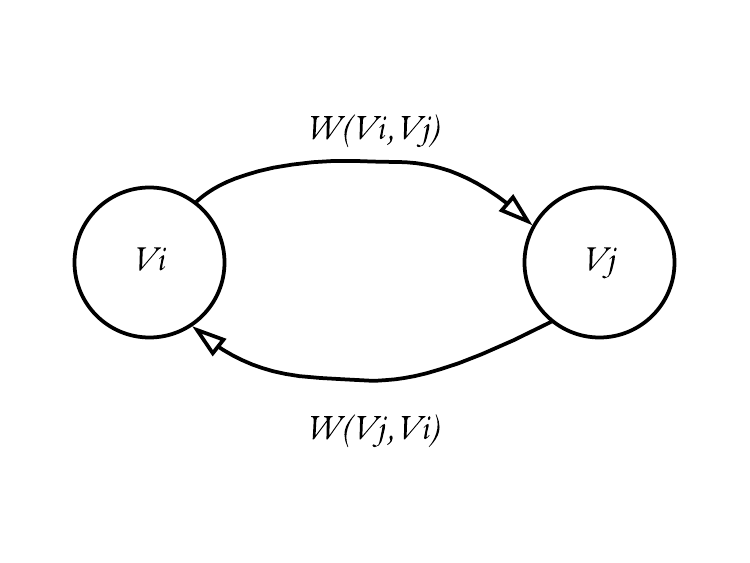
\includegraphics{images/graph}}
\caption{Graphical representation of developer's relations.}
\label{fig:graph}
\end{figure}

\subsection{Network Topology}
In order to apply this model on a real case scenario, we chose a OpenSource project to populate the network. Seeking a popular repository with reasonable amount of data, we look into official top-5 most reviewed projects\footnote{https://octoverse.github.com/}, selecting the one with most stars. This GitHub feature can be a measure of a project's passive community size\cite{sheoran2014}. These criteria pointed out to \textbf{Node.js}\footnote{https://github.com/nodejs/node}, a popular JavaScript runtime built on Chrome's V8 JavaScript engine. In order to understand the network behavior and evaluate if this is a reasonable representant of FOSS projects in this discussion, the following analyses were conducted. Table~\ref{tab:sizemetrics} shows Node's main size metrics.

\begin{table}[htbp]
\caption{Node.js Main Size Metrics}
\begin{center}
\begin{tabular}{|c|c|c|c|}
\hline
\textbf{Review Comments} & \textbf{Pullrequests}& \textbf{Stars}& \textbf{Contributors} \\
\hline
50.818 & 13.492 & 53.339 & 2.107 \\
\hline
\end{tabular}
\label{tab:sizemetrics}
\end{center}
\end{table}

Those features make Node.js one of the most active and influent project on GitHub. It's the 10th most stared JavaScript project, and the 24th globally\footnote{https://github.com/search?q=stars\%3A\%3E1&s=stars&type=Repositories}.

In order to discover how individuals interact on this network, its degree distribution was calculated. This relation is the probability distribution of individuals' degrees over the whole network. Since our network has directed edges, we compute outgoing degree, meaning the count of outgoing edges a node have. This represents how many individuals a particular node interacted with, showing his spreadness over the project. Fig.~\ref{fig:outdegree} shows the outdegree distribution of the proposed network. Based on this metric, often, these networks can be classified as random, free of scale, modular, small world, among others \cite{cross2004}. Since Fig.~\ref{fig:outdegree} shows that few individuals have the most connections, whereas the majority is only responsible for few relations, this can be described as free-scale network, with its outdegree distribution complying with the power law curve.


\begin{figure}[htbp]
\centerline{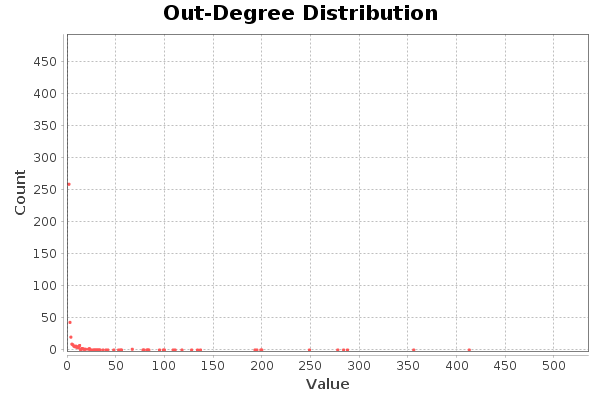
\includegraphics[width=\linewidth]{images/outdegree}}
\caption{Outdegree distribution}
\label{fig:outdegree}
\end{figure}

The edges are weighted, meaning the magnitude of each relationship in front of others author's interaction. Thus, Fig~\ref{fig:outdegree-weighted} shows the distribution also takes weight in consideration, giving a more accurate representation of influence distribution over the project. Considering recent contributions are more important to point out one's acbility to colaborate in actual matters, the influence gap grows even more. More than 94.6\% of the contributors have weighted outdegree lower than 1\% of the highest weighted outdegree. And only a little more than 4.5\% of all edges are between those individuals. This reinforces that the vast majority of interactions are made between core members or between regular contributors and core members.


\begin{figure}[htbp]
\centerline{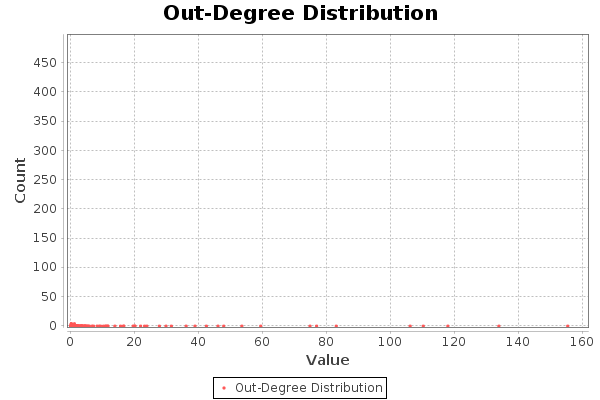
\includegraphics[width=\linewidth]{images/outdegree-weighted}}
\caption{Weighted outdegree distribution}
\label{fig:outdegree-weighted}
\end{figure}

Those metrics show that few individuals are responsible for most part of the discussion over contributions in this open source project. Those act as gatekeepers of project's goals and quality, guiding newcomers and evaluating the matter and content of community contributions. This structure seems to match earlier reported open source project's organization \cite{bergquist2001}. These experts can have knowledge and responsability over the project in general, or specialized in some modules \cite{firefox2018}, technologies or attributions \cite{debian2018}. Some projects do not have a formal division of core members responsability, but rather an informal distribution of tasks based on their availibility and expertise. This might be elucidated on community detection, as described in the next sessions.

\section{NetSCAN clustering algorithm}

The analysis of the network shows there are few individuals that hold great responsability over project's discussion and review, colaborating in higer proportion than the general community. Those also can be responsible for specifics, such as modules or technologies, even this is not formally defined in project's workflow documentation. Thus, it is important to identify them as they might be helpful for contributors on those specific topics, specially beginners that don't know where to start.

NetSCAN\cite{horta2018} is a density-based clustering algorithm, that extends the well known DBSCAN algorithm \cite{ester1996}. The main upgrade with respect to DBSCAN is that NetSCAN considers the edge's direction between two nodes. Other important difference is that NetSCAN also can detect that a individual can be in more than one group. Hence we are searching for informal, blurred and often tenuous expertise and responsability distributions, NetSCAN suits our goals better. NetSCAN identifies each cluster cores, wich can also be overlapped.

NetSCAN receives two parameters, \textit{eps} and \textit{minPts}. While the former represents the edge's minimal weight consider that relationship on the clustering process, \textit{minPts} is the threshold where only individuals with higher pontuaction can be considered as core members. In order to find suitable parameter configuration, we tested different combinations seeking for optimizing the clusters's silhouette~\cite{tan2005}. This metric use the distance between nodes to account their similarity. The idea behind it is that individuals inside a cluster should be closer to its companions than to outsiders. The index variates from -1 to 1, and higher values mean that interactions inside the cluster are strong than outside edges~\cite{almeida2011}.

To evaluate the silhouette of each configuration, we chose minimal and maximal \textit{eps} and \textit{minPts} values, with a \textit{step size} value for each, as stated on Table~\ref{tab:configparams}. the \textbf{Set Size} column means how many configuration possibilities will be generated by the variaton step by step from min to max values.

\begin{table}[htbp]
\caption{Configuration Parameters to maximize silhouette}
\begin{center}
\begin{tabular}{|c|c|c|c|c|}
\hline
\textbf{Parameter} & \textbf{Min}& \textbf{Max}& \textbf{Step Size} & \textbf{Set Size} \\
\hline
\textit{eps} & 0.20 & 1.0 & 0.05 & 16 \\
\hline
\textit{minPts} & 20 & 130 & 10 & 11 \\
\hline
\end{tabular}
\label{tab:configparams}
\end{center}
\end{table}

Lowest values $eps=0.20$ and $minPts=20$ were chosen because they are roughly the firsts to generate more than one cluster. Highest $eps=1.0$ is setted because it is the grater weight an edge can have, while $minPts=130$ is roughly second higher weighted outdegree, meaning higher \textit{minPts} would oblige that only one core could exist. Those two sets combined gave us 176 tuples, that were dinamically tested. The higher silhouette was X, by the combination $eps=A$ and $minPts=B$. More details will be shown in the next section.

NetSCAN is also bundled as a Neo4j plugin\footnote{https://github.com/vitorhorta/netscan-neo4j}, and can be runned directly from Cypher queries with dinamic parameters.

\section{Results}

The project data was loaded into the network, with help of neo4j graph database. Not all of contributors counted on Table~\ref{tab:sizemetrics} were loaded, since some never opened or reviewed a pullrequest and only helped opening or replying to issues. Table 1 shows result's summary of the clustering process.

\begin{table}[htbp]
\caption{Main project}
\begin{center}
\begin{tabular}{|c|c|c|c|c|}
\hline
\textbf{Nodes} & \textbf{Clusterized}& \textbf{Overlapped} & \textbf{Clusters} & \textbf{Cores} \\
\hline
1.444 & 969 & 324 & 13 & 16 \\
\hline
\end{tabular}
\label{tab:sizemetrics}
\end{center}
\end{table}

\subsection{Future Work}

\subsection{Conclusions}

\section*{References}
\bibliographystyle{IEEEtran}
\bibliography{../bibrefs/refs}

\end{document}
